% !TEX root =./main.tex

\section{Signal $x_1$}

Signal $x_1$ contains two tones.  The louder tone (Tone 1) is at approximately $1539 \unit{Hz}$, and the quieter (Tone 2) at $2000$.  The tones can be seen in the signal's frequency spectrum in Figure \ref{fig:X1}.  The unfiltered audio can be heard with the \code{x1\_unfiltered.wav} file in the \href{https://github.com/dbcometto/ece434_cpx2}{GitHub repository}.

\begin{figure}[H]
    \centering
    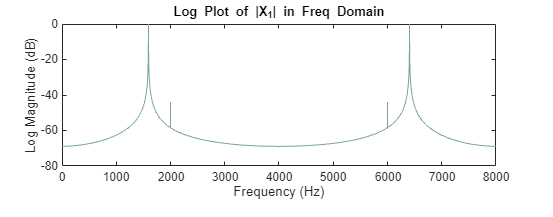
\includegraphics[width=0.5\linewidth]{figures/X1.png}
    \caption{Signal $x_1$ Frequency Spectrum}
    \label{fig:X1}
\end{figure}

In Figure \ref{fig:x1} and Figure \ref{fig:x1_zoom}, the signal can be seen in the time domain.  The signal looks as expected for two sinusoids being present, although the effect of Tone 2 is minimal.

\begin{figure}[H]
    \centering
    \includegraphics[width=0.5\linewidth]{figures/x1.png}
    \caption{Signal $x_1$ by Time}
    \label{fig:x1}
\end{figure}

\begin{figure}[H]
    \centering
    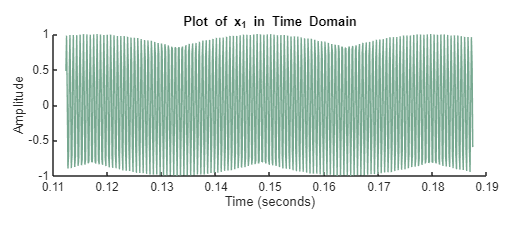
\includegraphics[width=0.5\linewidth]{figures/x1_zoom.png}
    \caption{Signal $x_1$ by Time}
    \label{fig:x1_zoom}
\end{figure}

Before any filtering is done, we can calculate the period of the dominant sinusoid.  From the frequency spectrum, we see that
\begin{align*}
    T = \frac{1}{1593 \unit{Hz}} = 620 \unit{$\micro$s},
\end{align*}
and from the plot in Figure \ref{fig:x1_timeT},
\begin{align*}
    T = 0.147625 \unit{s} - 0.147 \unit{s} = 625 \unit{$\micro$s}.
\end{align*}

\begin{figure}
    \centering
    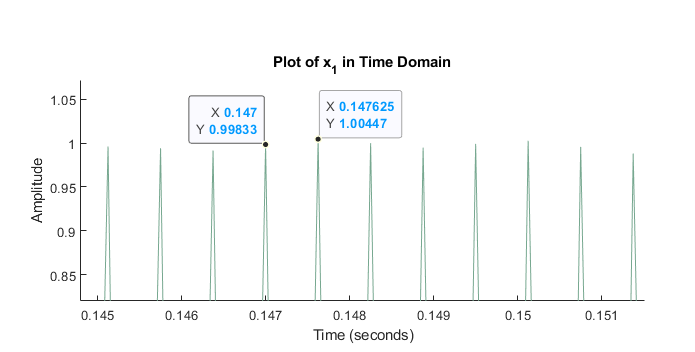
\includegraphics[width=0.5\linewidth]{figures/x1_timeperiod.png}
    \caption{Signal $x_1$ by Time with few Cycles}
    \label{fig:x1_timeT}
\end{figure}

The processing goal for Signal $x_1$ was to attenuate the tone of higher magnitude (Tone 1) so that the magnitude of Tone 1 was more than $30 \unit{dB}$ less than the magnitude of the tone of lower magnitude (Tone 2).  

A highpass filter was chosen for the first method, as that was the simplest option.  Because preserving linear phase is not important, IIR was chosen.  Additionally, the elliptic method was chosen as it yields the best magnitude response for a given order.  After several iterations, Filter 1 with the parameters in Table \ref{tab:x1_v2} was designed.

\begin{table}[H]
    \centering
    \begin{tabular}{c|cccc}
         Order & Fstop & Fpass & Astop & Apass \\ \hline
         7 & $1600  \unit{Hz}$ & $2000  \unit{Hz}$ & $73  \unit{dB} $ & $1  \unit{dB}$
    \end{tabular}
    \caption{Parameters for Filter 1 for Signal $x_1$}
    \label{tab:x1_v2}
\end{table}

Applying this filter to the signal yielded the response in Figure \ref{fig:X1_v2}.  The horizontal dark green line marks $-30\unit{dB}$, with the peak of Tone 2 at $0 \unit{dB}$.  Because the magnitude of Tone 1 is more than $30 \unit{dB}$ less than the magnitude of Tone 2, Filter 1 meets the specifications at order 7.  The signal's response can be heard with the \code{x1\_filtered7.wav} file in the \href{https://github.com/dbcometto/ece434_cpx2}{GitHub repository}.

\begin{figure}[H]
    \centering
    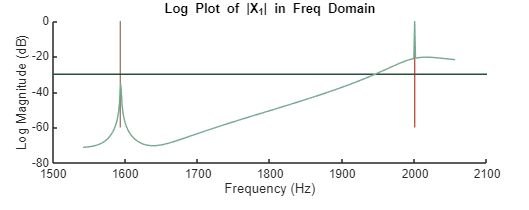
\includegraphics[width=0.5\linewidth]{figures/X1_filterv2.png}
    \caption{Response of Signal $x_1$ to Filter 1, Order 7}
    \label{fig:X1_v2}
\end{figure}

In order to reduce the order, a notching filter's poles and zeros were modified.  An order 2 filter, with a zero on Tone 1's frequency, was unable to reduce the magnitude enough.  Thus, Filter 2, an order 4 filter with the pole zero plot in Figure \ref{fig:x1_v10_polezero} was developed.

\begin{figure}[H]
    \centering
    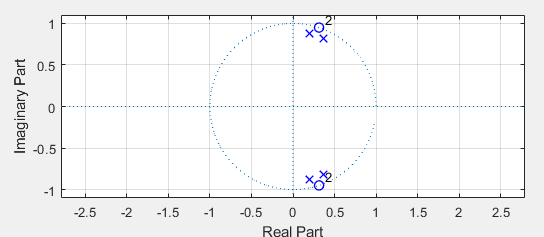
\includegraphics[width=0.5\linewidth]{figures/x1_v10_polezero.png}
    \caption{Pole Zero Plot of Filter 2 for Signal $x_1$}
    \label{fig:x1_v10_polezero}
\end{figure}

The locations of the poles and zeros are recorded in Table \ref{tab:x1_v10}.

\begin{table}[H]
    \centering
    \begin{tabular}{c|cccc}
         Order & & Zeros & Pole & Pole \\ \hline
         4 & Angle & $\pm 1.2519 \unit{rad}$  & $\pm 1.1519 \unit{rad}$ & $\pm 1.3519 \unit{rad}$ \\
         & Magnitude & $1$ & $0.9$ & $0.9$
    \end{tabular}
    \caption{Parameters for Filter 2 for Signal $x_1$}
    \label{tab:x1_v10}
\end{table}

The signal response of Filter 2 can be seen in Figure \ref{fig:X1_v10}.  The signal response can be heard in the \code{x1\_filtered4.wav} file in the \href{https://github.com/dbcometto/ece434_cpx2}{GitHub repository}.

\begin{figure}[H]
    \centering
    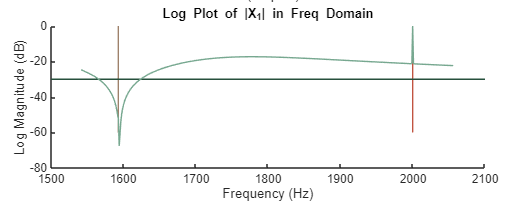
\includegraphics[width=0.5\linewidth]{figures/X1_filterv10.png}
    \caption{Response of Signal $x_1$ to Filter 2, Order 4}
    \label{fig:X1_v10}
\end{figure}

Because of the sharpness of the notching filter, the response looks different than expected for two tones.  Additionally, the sound is not identical to the first response.  Despite these factors, the majority of Tone 1's magnitude is below the $-30 \unit{dB}$ line, and thus Filter 2 meets the specifications with order 4.

The response of an order 2 notching filter can be seen in Figure \ref{fig:X1_v11}.  The filter is not able to bring Tone 1's magnitude below the $-30\unit{dB}$ specification.

\begin{figure}[H]
    \centering
    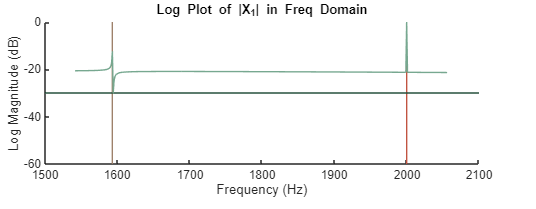
\includegraphics[width=0.5\linewidth]{figures/X1_filterv11.png}
    \caption{Response of Signal $x_1$ to an Order 2 Notching Filter}
    \label{fig:X1_v11}
\end{figure}

After filtering, we can again calculate the period of the dominant sinusoid.  From the frequency spectrum, we see that
\begin{align*}
    T = \frac{1}{2000 \unit{Hz}} = 500 \unit{$\micro$s},
\end{align*}
and from the plot in Figure \ref{fig:x1_timeT2},
\begin{align*}
    T = 0.207125 \unit{s} - 0.206625 \unit{s} = 500 \unit{$\micro$s}.
\end{align*}

\begin{figure}
    \centering
    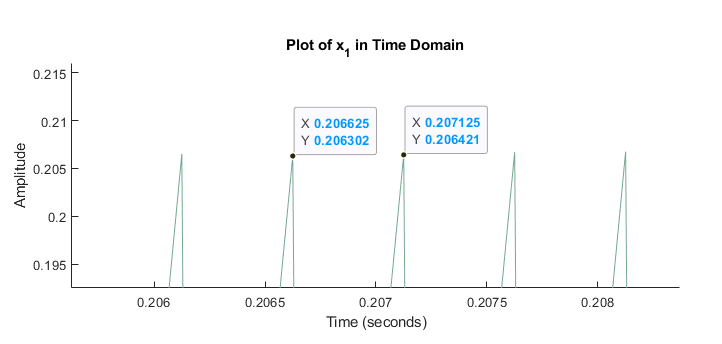
\includegraphics[width=0.5\linewidth]{figures/x1_timeperiod2.png}
    \caption{Signal $x_1$ After Filtering by Time with few Cycles}
    \label{fig:x1_timeT2}
\end{figure}